% \section{Performance Evaluation and Analysis}

Performance analysis is a systematic study and measurement of various performance metrics to determine the effectiveness and efficiency of a system, process, or application. This includes factors such as processing speed (latency), memory utilization, and power consumption

This chapter focuses on the quantitative assessment of performance metrics, specifically processing speed, memory requirements, and power consumption. The objective of this chapter is to compare two distinct algorithms: one based on a lightweight algorithm and the based on a traditional heavyweight encryption algorithm. This comparative analysis is conducted both at the functional level and within the broader application context of the proposed solution.

Before we start the analysis, we present a case scenario that serves as the foundation for our measurements. Subsequently, the chapter reveals the outcomes of our performance measurements, shedding light on the quantitative results derived from the analysis. Last, we delve into a security analysis of the proposed communication scheme. This evaluation aims to validate the robustness and reliability of the proposed communication scheme, thereby ensuring its effectiveness in real-world scenarios.


% This chapter discusses the quantitative assessment of performance metrics such as processing speed(latency), memory requirement, and power consumption. It has a primary  objective of comparing two distinct algorithms; one based on a lightweight and the other based on a heavyweight; both at the function level and within the broader application context of the proposed solution. 

% we first presented the case scenario of the measurement and then the performance measurement result. Last, the security analysis of the scheme is provided to validate the robustness of the proposed communication scheme. 

\section{Measurement Case Scenarios}

To measure the performance of our proposed solution, we prepared three case scenarios. For each case scenario, we also performed analysis from the algorithm (function call ) perspective and running application overhead. 

\textit{Case 1: AES-GCM} - In this case, the performance AES-GCM encryption algorithm is tested in terms of power, memory, and speed. First, its solo impact - as function -  and then implementation based on this algorithm from the application level is analysed.


\textit{Case 2: ASCON} - Similarly, in this case, the ASCON encryption algorithm both at function and its impact on the implementation of the proposed solution is measured. 

\textit{Case 3: No encryption} - This case scenario was used as a baseline reference for the other two cases. In this case, we called a function that has a similar signature to the encryption function calls we used for ASCON and AES-GCM. However, the underlying function did not perform any operation other than copying values from one memory to another. The implementation code for this case can be seen in the following code list.

\begin{lstlisting}[style=CStyle, caption={C Implementation Of No-Encryption - Base Line Reference of Measurement}, label={list:no-enc}]
int crypto_aead_encrypt(
      unsigned char *c,unsigned long long *clen,
      const unsigned char *m,unsigned long long mlen,
      const unsigned char *ad,unsigned long long adlen,
      const unsigned char *nsec,
      const unsigned char *npub,
      const unsigned char *k
      )
{
  *clen = mlen + CRYPTO_ABYTES;
  memcpy(c, m, mlen);
  memset(c + mlen, 0, CRYPTO_ABYTES);

  return 0;
}

int crypto_aead_decrypt(
  unsigned char *m, unsigned long long *mlen,
  unsigned char *nsec,
  const unsigned char *c, unsigned long long clen,
  const unsigned char *ad, unsigned long long adlen,
  const unsigned char *npub,
  const unsigned char *k
)
{
  unsigned long long len = *mlen = clen - CRYPTO_ABYTES;
  memcpy(m, c, len);

  return 0;
} 
\end{lstlisting}


\section{Performance measurement - Speed, Memory, and Power}
Depending on the complexity of an algorithm (process round) and the required CPU instruction (operation) there shall be differences in performance between various categories of algorithms. However, it is important to note that there is a trade-off between security and performance. Hence, prior to selecting an algorithm, designers and practitioners need to carefully evaluate the minimal required security level for a given application. 

This section aims to offer insight into the performance of two specific algorithms, namely AES and ASCON. In both algorithms, the same key size is used. Our focus lies on measuring their processing speed, memory consumption, and power utilization. Furthermore, to establish a benchmark, we incorporate a non-encrypted implementation for comparison purposes.

\subsection{Speed - Running Time}
% execution time 
% 
In the Arduino ESP-IDF framework, we measure the execution time of a function using the built-in functions provided by the framework. The \texttt{esp\_timer\_get\_time()} function is used to retrieve the current time in microseconds since the underlying device boot. By capturing the start time before executing the function and the end time after the function completes, we calculate the execution time by subtracting the start time from the end time.

Our experimental setup involves three distinct case scenarios. Firstly, we measure the execution time when the application runs without any encryption algorithm. Then, we measure the execution time when the messages are encrypted using ASCON and AES algorithms. Note that we measure the performance of the proposed solution from two perspectives; 1) From the time required to run the encryption algorithm within the application program and 2) from the perspective of measuring the total time required to process the message and send it to the digital twin (Cloud). Both case scenarios are shown in figure Fig \ref{Fig:time-scheme} and Fig \ref{Fig:time-algorithm}. 

To obtain accurate measurements, we allow our programs to run 1000 function calls sending data after encryption for each case scenario. We then calculate the average execution time using a Python script that processes the dump file we collected from the device.

As it can be seen from Figure \ref{Fig:time-algorithm} ASCON's execution time is lower than AES-GCM. Similarly, Figure \ref{Fig:time-scheme} shows that our proposed solution performs well when ASCON is used. These results suggest that ASCON is a promising candidate for use in our proposed solution.

\begin{figure}[H]
        % \centering
        \begin{subfigure}[c]{0.48\linewidth}
            \resizebox{\linewidth}{!}{
                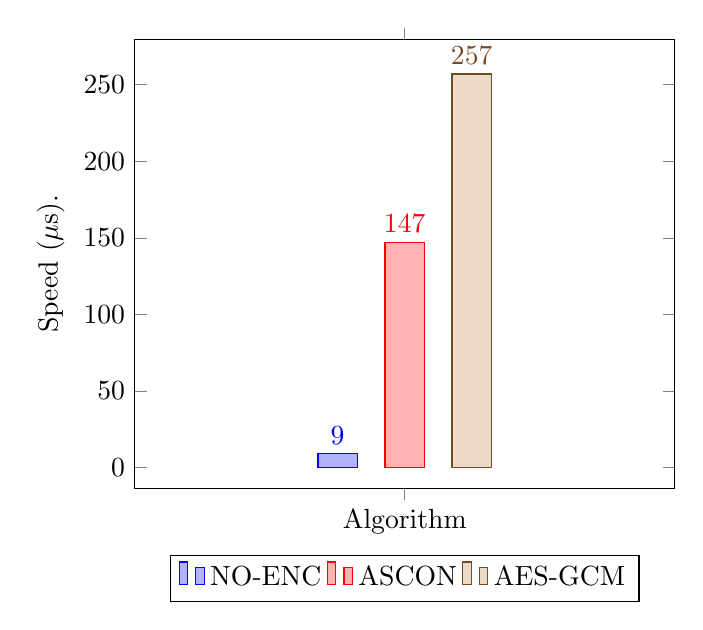
\begin{tikzpicture}
                    \begin{axis}[
                        ybar = 10pt,
                        enlargelimits=0.09,
                        legend style={at={(0.5,-0.15)},
                        anchor=north,legend columns=-1},
                        ylabel={Speed ($\mu$s).},
                        symbolic x coords={Algorithm, Scheme},
                        xtick=data,
                        nodes near coords,
                        nodes near coords align={vertical},
                        bar width = 0.5cm,
                        ]
                        \addplot coordinates {(Algorithm,9)};
                        \addplot coordinates {(Algorithm,147)};
                        \addplot coordinates {(Algorithm,257)};
                        % \addplot coordinates {(Algorithm,2)};
                         
                        \legend{NO-ENC, ASCON, AES-GCM}
                    \end{axis}
                \end{tikzpicture}
            }
        \caption{Speed From The Algorithm Execution Perspective ($\mu$s).}
        \label{Fig:time-algorithm}
    \end{subfigure}%
    \begin{subfigure}[c]{0.48\linewidth}
        \resizebox{\linewidth}{!}{
            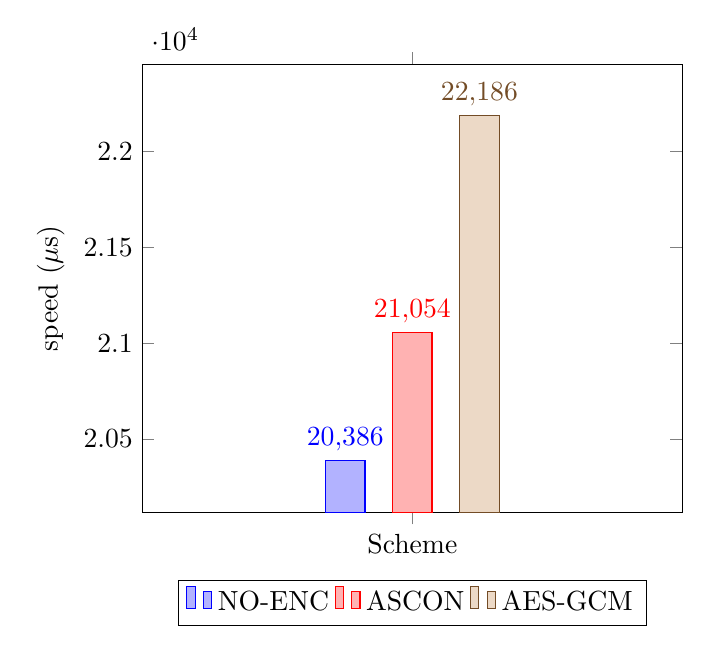
\begin{tikzpicture}
                \begin{axis}[
                    ybar = 10pt,
                    enlargelimits=0.15,
                    legend style={at={(0.5,-0.15)},
                    anchor=north,legend columns=-1},
                    ylabel={speed ($\mu$s)},
                    symbolic x coords={Scheme},
                    xtick=data,
                    nodes near coords,
                    nodes near coords align={vertical},
                    bar width = 0.5cm,
                    ]
                    \addplot coordinates {(Scheme,20386)};
                    \addplot coordinates {(Scheme,21054)};
                    \addplot coordinates {(Scheme,22186)};
                    % \addplot coordinates {(Algorithm,2)};
                     
                    \legend{NO-ENC, ASCON, AES-GCM}
                \end{axis}
            \end{tikzpicture}
            }
    \caption{Speed From The Scheme (Application) Perspective ($\mu$s)}
    \label{Fig:time-scheme}
\end{subfigure}
\caption{Performance Of Three Case Scenarios From Algorithm Execution Speed and Application Running Time.}
\label{Fig:perform-speed}
\end{figure}

\subsubsection*{Throughput and Cycle Byte Ratio}

Throughput is a performance indicator of a system that measures the number of bytes processed per unit of time (typically seconds). It is a measure of how efficiently a system can process data. The more bytes that are processed per unit of time, the better the system performs. Throughput is typically measured in bytes per second (Bps) or kilobytes per second (Kbps).

The Cycle Byte Ratio is another performance metric that measures the number of CPU cycles needed to process a single byte. Table \ref{tbl:cycle-count} presents the cycle counts for different scenarios: 1) without employing any encryption algorithm, 2) utilizing the ASCON encryption algorithm, and 3) employing the AES-GCM encryption algorithm.


\begin{table}[H]
    \tiny
    \centering
    \caption{Cycle Count For 3 Cases: No-Encryption, ASCON, AES-GCM }
    \label{tbl:cycle-count}
    \resizebox{0.8\textwidth}{!}
    {
        \begin{tabular}{l | a | b | a}
        \hline
        \rowcolor{LightCyan}
        \mc{1}{}  & \mc{1}{No-Encryption}  & \mc{1}{ASCON} & \mc{1}{AES-GCM}\\
        \hline
        Cycle Count & 2009 & 36811  &  49956\\
        Byte Processed & 32  & 32 &  32\\ 
        CPU Freq MHz & 240 & 240 &  240\\ 
        Cycle per Byte &  64.28 & 1094.68 &  31517.90\\ 
        Time Elapsed $\mu$s & 8.57  & 145.95 &  202.38\\ 
        Throughput B/$\mu$s & 3.73  & 0.219 &  0.158\\ 
        \hline
        \end{tabular} 
        }
\end{table}

\begin{equation}
\text{Throughput} = \frac{\text{Byte processed}}{\text{Total Time}} \quad \text{Cycle Byte} = \frac{\text{Cycle Count}}{\text{Byte processed}}
\label{eq:4.1}
\end{equation}

The total time taken by the CPU to perform an operation can be derived using cycle count and the CPU clock frequency. The total time taken by the operation is equal to the cycle count multiplied by the CPU clock frequency. 

To calculate the throughput and the cycle byte ratio for each algorithm in our proposed solution, we use 64 bytes of data as input. Figure \ref{tbl:cycle-count}

\begin{equation}
\text{Total Time} = \frac{\text{Cycle Count}}{\text{CPU frequency in Mhz/Khz}}
\label{eq:4.2}
\end{equation}

In this experiment, while we use \texttt{$xthal\_get\_ccount()$} from esp32/ck.h library to get the cycle count at a given time, we use \texttt{$getCpuFrequencyMhz()$} function to get the current set CPU frequency of the device fro esp32-hal-cpu.c source file.  

We calculated the throughput and cycle byte ratio of each algorithm in the proposed solution processing 16 bytes of message and 16 bytes of associated data, using equation \ref{eq:4.1}. The results are shown in Figures \ref{fig:put} and\ref{fig:ccb-ratio}


\begin{figure}[H]
        % \centering
        \begin{subfigure}[c]{0.48\linewidth}
            \resizebox{\linewidth}{!}{
                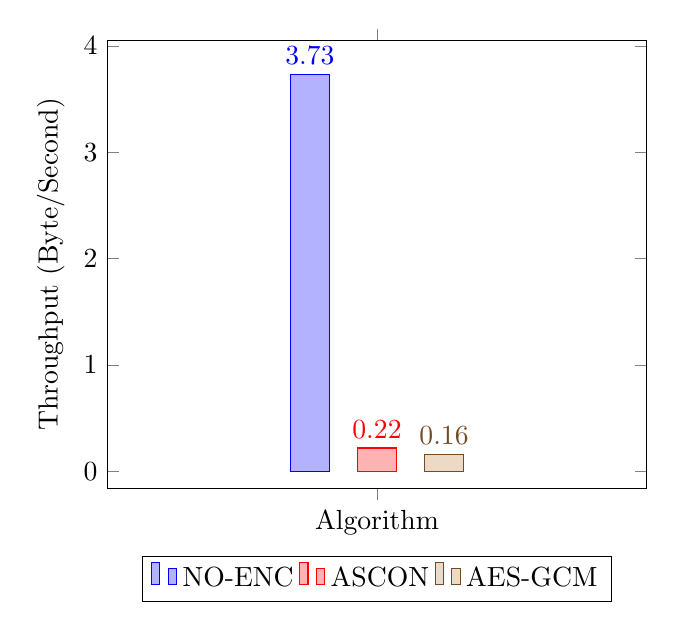
\begin{tikzpicture}
                    \begin{axis}[
                        ybar = 10pt,
                        enlargelimits=0.09,
                        legend style={at={(0.5,-0.15)},
                        anchor=north,legend columns=-1},
                        ylabel={Throughput (Byte/Second)},
                        symbolic x coords={Algorithm},
                        xtick=data,
                        nodes near coords,
                        nodes near coords align={vertical},
                        bar width = 0.5cm,
                        ]
                        \addplot coordinates {(Algorithm,3.73)};
                        \addplot coordinates {(Algorithm,0.219)};
                        \addplot coordinates {(Algorithm,0.158)};
                         
                        \legend{NO-ENC, ASCON, AES-GCM}
                    \end{axis}
                \end{tikzpicture}
            }
        \caption{Throughput of the algorithms (Bytes/Seconds).}
        \label{fig:put}
    \end{subfigure}%
    \begin{subfigure}[c]{0.48\linewidth}
        \resizebox{\linewidth}{!}{
            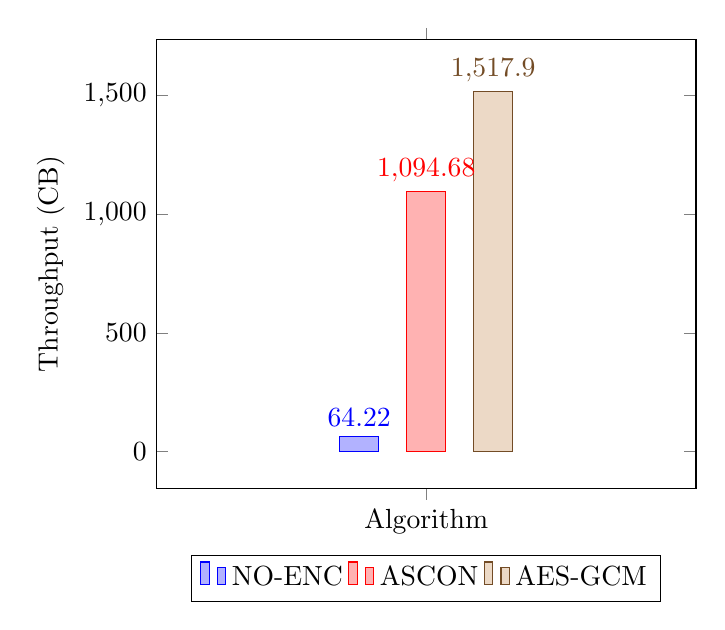
\begin{tikzpicture}
                \begin{axis}[
                    ybar = 10pt,
                    enlargelimits=0.15,
                    legend style={at={(0.5,-0.15)},
                    anchor=north,legend columns=-1},
                    ylabel={Throughput (C\\B)},
                    symbolic x coords={Algorithm},
                    xtick=data,
                    nodes near coords,
                    nodes near coords align={vertical},
                    bar width = 0.5cm,
                    ]
                    \addplot coordinates {(Algorithm,64.218)};
                    \addplot coordinates {(Algorithm,1094.68)};
                    \addplot coordinates {(Algorithm,1517.90)};
                    % \addplot coordinates {(Algorithm,2)};
                     
                    \legend{NO-ENC, ASCON, AES-GCM}
                \end{axis}
            \end{tikzpicture}
            }
    \caption{Throughput In Cycle per Byte ratio.}
    \label{fig:ccb-ratio}
\end{subfigure}
\caption{Throughput and cycle per byte ratio of each algorithms.}
\label{Fig:throughput-cycle}
\end{figure}


% ****************************************************************************************
\subsection{Static and Dynamic Memory Footprint }
% show the ram and flash memory of embeded progrma 
Analyzing and measuring the memory usage of embedded programs is vital, especially when the device has memory constraints. In this section, we will discuss the static and dynamic memory usage of our proposed solution. Throughout our measurement, we compared three implementations scenarios:
\begin{itemize}
    \item No encryption,
    \item Encryption using ASCON, and
    \item Encryption using AES-GCM
\end{itemize}

\begin{figure}[H]
    \centering
    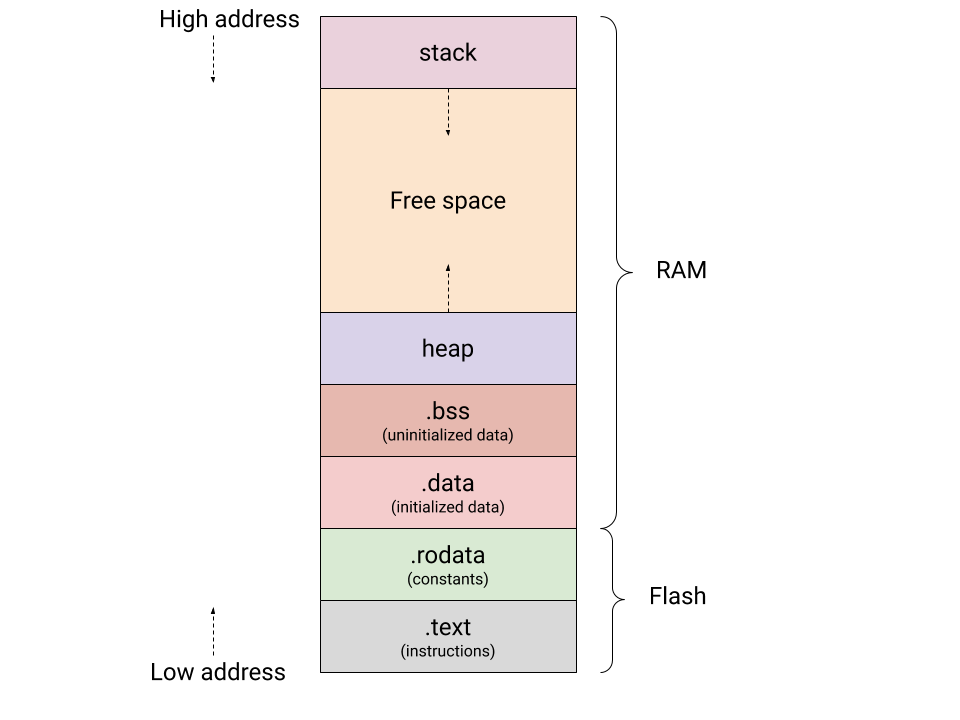
\includegraphics[width=0.8\linewidth]{images/fp/memory-analysis.png}
    \caption{Memory Map of Embedded Programming (taken from \cite{koval_analyze_2020})}
    \label{fig:memory-map}
\end{figure}

Figure \ref{fig:memory-map} depicts the general memory map of embedded programming. The flash part of the memory that includes the .rodata and .text section contains the code resulting from compiling and building the source program. This section contains static codes and requires a fixed memory size. Whereas, the RAM section of the memory is responsible for containing a few sections for statically generated codes and the majority one for handling dynamic memory management such as stack and heap allocation.


In our analysis of the dynamic memory usage for our implementation of the proposed solution, we focused only on the RAM section. However, when assessing the static memory usage (code size), we examined both the RAM and Flash sections. This approach was necessary as both sections contribute to the overall code size. 

\subsubsection*{Static Memory Usage - Code size}
% Provide a table 
% Draw a graph 

The static code size measurement was conducted to compare the code size requirements of three different implementation scenarios: No-Encryption, ASCON, and AES-GCM. The goal was to assess the impact of these implementations on resource-constrained devices in terms of memory usage.

Table \ref{tbl:ins-codesize} provides a summary of the code size measurements for each scenario. In the No-Encryption scenario, no additional code was required beyond the base program, resulting in minimal memory usage. Our implementation based on ASCON introduced a slight increase in code size. Approximately 1 KB of additional memory was needed in both RAM and Flash compared to the No-Encryption scenario. On the other hand, AES-GCM demonstrated slightly higher code size requirements. The implementation demanded approximately 8 KB more RAM and 5.6 KB more Flash memory compared to the No-Encryption case.


\begin{table}[H]
    \tiny
    \centering
    \caption{Code Size (KB): No-Encryption, ASCON, AES-GCM }
    \label{tbl:ins-codesize}
    \resizebox{0.8\textwidth}{!}
    {
        \begin{tabular}{l | a | b | a}
        \hline
        \rowcolor{LightCyan}
        \mc{1}{}  & \mc{1}{No-Encryption}  & \mc{1}{ASCON} & \mc{1}{AES-GCM}\\
        \hline
        Ram \/KB & 59.3 & 59.3  &  68\\
        Flash KB & 766.5  & 767.7 &  772.1\\ 
        Total KB & 825.8 & 827 &  840.1\\ 
        % Cycle per Byte &  64.28 & 1094.68 &  31517.90\\ 
        % Time Elapsed $\mu$s & 8.57  & 145.95 &  202.38\\ 
        % Throughput B/$\mu$s & 3.73  & 0.219 &  0.158\\ 
        \hline
        \end{tabular} 
        }
\end{table}

\begin{figure}[H]
    \centering
    
    \resizebox{0.45\textwidth}{!}
    {
        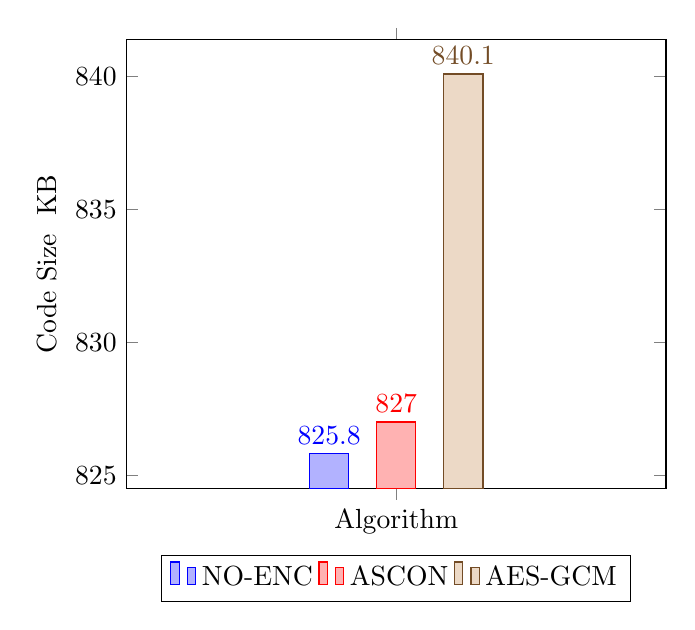
\begin{tikzpicture}
            \begin{axis}[
                ybar = 10pt,
                enlargelimits=0.09,
                legend style={at={(0.5,-0.15)},
                anchor=north,legend columns=-1},
                ylabel={Code Size \/ KB},
                symbolic x coords={Algorithm},
                xtick=data,
                nodes near coords,
                nodes near coords align={vertical},
                bar width = 0.5cm,
                ]
                \addplot coordinates {(Algorithm,825.8)};
                \addplot coordinates {(Algorithm,827)};
                \addplot coordinates {(Algorithm,840.1)};
                 
                \legend{NO-ENC, ASCON, AES-GCM}
            \end{axis}
        \end{tikzpicture}   
    }
    \caption{Static Code Size of The Scheme For 3 Scenarios(No-Encryption, ASCON, AES-GCM}
\label{Fig:codesize}
\end{figure}



\subsubsection*{Dynamic RAM Usage}

% I will explain the techniques I used to capture the memory usage
% The challenge of measuring the memory heap 
% Explain or provide an analysis of memory for each case 

Measuring the dynamic RAM usage of each algorithm is not as easy as measuring static memory usage. The heap and stack are two types of dynamic memory, making it challenging to keep track of their usage as they are allocated and freed during function calls and returns. One effective technique recommended by NIST is to overwrite the memory with known values before running the program and keep track of the memory cells that are overwritten by the program. However, due to the complexity of setting it up,  we decided to employ alternative techniques to approximate the dynamic memory usage of each algorithm described as follows.



In our device (ESP32), we discovered that the initially allocated memory for handling heap and stack allocation is 327,680 Bytes. Having this in mind, we track the minimum heap size ever available, utilising the system call \textit{esp\_get\_minimum\_free\_heap\_size}. Our program was executed for 1000 iterations calling the encryption function for each implementation, allowing us to obtain a snapshot of the free memory available between the stack and heap 1000 times. By calculating the difference between the total allocated dynamic memory and the minimum heap size recorded, we were able to approximate the memory footprint of each implementation.

Furthermore, we employed the baseline implementation, which does not incorporate an encryption/decryption algorithm, as a benchmark to estimate the dynamic memory usage overhead added by ASCON and AES-GCM algorithms(see Fig \ref{Fig:memory-algo}). This comparison with the baseline provided insight into the dynamic memory usage of each algorithm at the running time. 

\begin{figure}[H]
        % \centering
        \begin{subfigure}[c]{0.48\linewidth}
            \resizebox{\linewidth}{!}{
                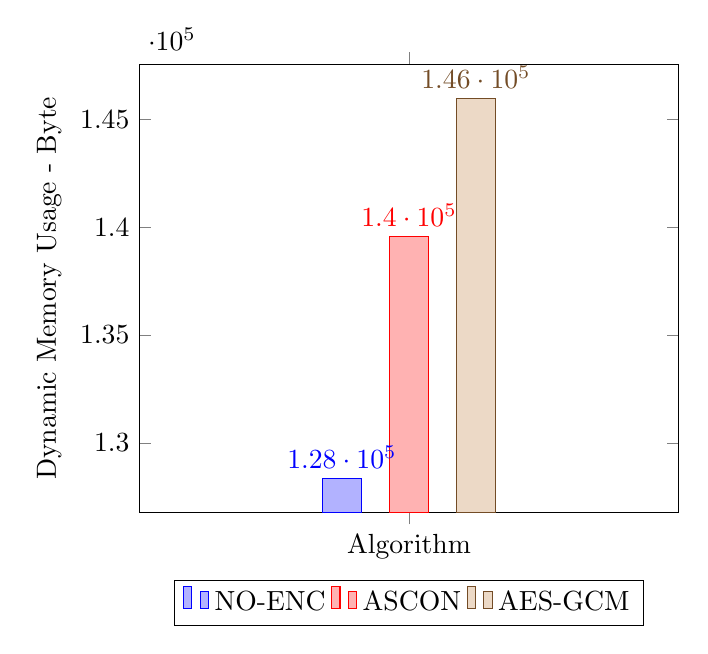
\begin{tikzpicture}
                    \begin{axis}[
                        ybar = 10pt,
                        enlargelimits=0.09,
                        legend style={at={(0.5,-0.15)},
                        anchor=north,legend columns=-1},
                        ylabel={Dynamic Memory Usage - Byte},
                        symbolic x coords={Algorithm},
                        xtick=data,
                        nodes near coords,
                        nodes near coords align={vertical},
                        bar width = 0.5cm,
                        ]
                        \addplot coordinates {(Algorithm,128356)};
                        \addplot coordinates {(Algorithm,139588)};
                        \addplot coordinates {(Algorithm,145972)};
                         
                        \legend{NO-ENC, ASCON, AES-GCM}
                    \end{axis}
                \end{tikzpicture}
            }
        \caption{Heap and Stack Memory Usage Each Implementation.}
        \label{Fig:dynamic-memory}
    \end{subfigure}%
    \begin{subfigure}[c]{0.48\linewidth}
        \resizebox{\linewidth}{!}{
            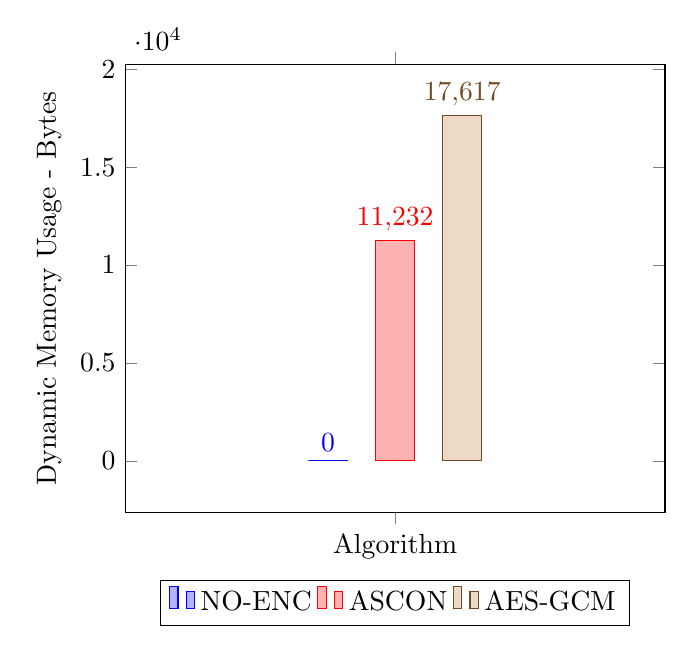
\begin{tikzpicture}
                \begin{axis}[
                    ybar = 10pt,
                    enlargelimits=0.15,
                    legend style={at={(0.5,-0.15)},
                    anchor=north,legend columns=-1},
                    ylabel={Dynamic Memory Usage - Bytes},
                    symbolic x coords={Algorithm},
                    xtick=data,
                    nodes near coords,
                    nodes near coords align={vertical},
                    bar width = 0.5cm,
                    ]
                    \addplot coordinates {(Algorithm,0)};
                    \addplot coordinates {(Algorithm, 11232)};
                    \addplot coordinates {(Algorithm, 17617)};
                    % \addplot coordinates {(Algorithm,2)};
                     
                    \legend{NO-ENC, ASCON, AES-GCM}
                \end{axis}
            \end{tikzpicture}
            }
    \caption{The Additional Memory Overhead Introduced by the Algorithm.}
    \label{Fig:memory-algo}
\end{subfigure}
\caption{Dynamic Memory Usage Comparison of Our Scheme Implementation and Algorithms}
\label{Fig:memory-impl-algo}
\end{figure}

\subsection{Power Consumption Measurement }
\label{sec:power}
Power consumption is a critical factor for low-power (I)IoT devices, as it can affect their battery life. There are a number of methods for measuring the power consumption of (I)IoT devices including using a USB power meter and Oscilloscope. while the former method can be inaccurate, as it does not account for the power consumption of individual components in the device, the latter method is more accurate as it uses a current probe to measure the current draw of CPU, memory, and other component individually. In this section, we provide the methods and results of power measurement for ESP32. 

\subsubsection*{Method of Power Measurement}
Measuring the power consumption of an algorithm or running application is a very challenging task due to the power noises stemming from other board components, such as Wi-Fi and Bluetooth \cite{noauthor_current_nodate}. Getting a precise power consumption of running machine code on a chip requires a carefully set up lab environment, where the chip is isolated from the other components. This procedure involves connecting a fine-grained voltage source, typically an expensive oscilloscope, and capturing and measuring the power intake to the chip.

\begin{figure}
    \centering
    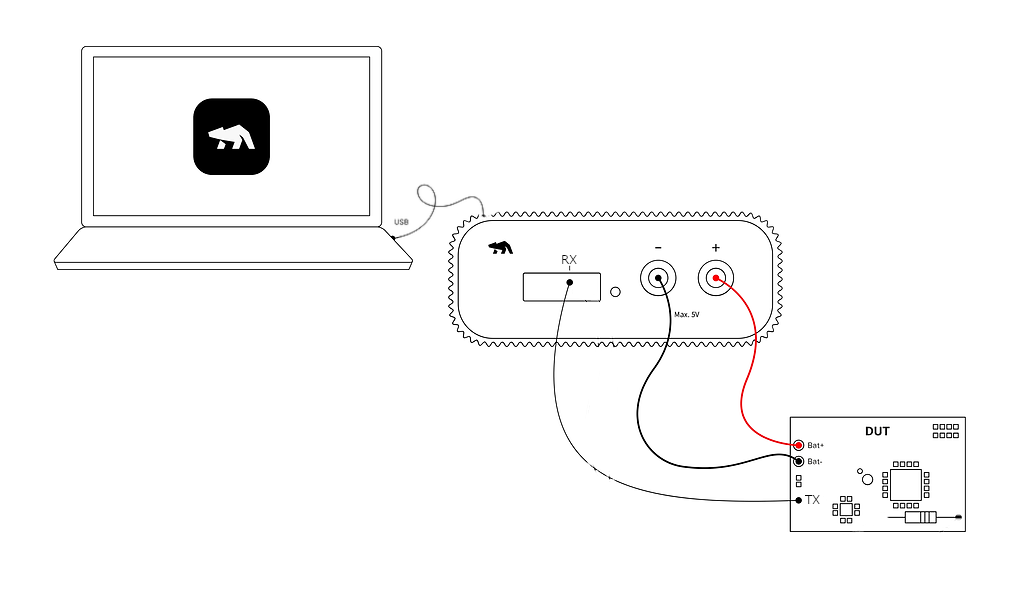
\includegraphics[width=0.9\textwidth]{images/fp/otii-uart-log.png}
    \caption{Power Measurement Setup Using Otii-arch.}
    \label{fig:otii-pow}
\end{figure}
However, in this project, we approximate the power consumption of our proposed solution using Otti arch from Quitech AB \footnote{\url{https://www.qoitech.com/otii-arc-pro/} A versatile instrument that sources voltage or current, measures both simultaneously, and helps optimize battery life by identifying energy-draining factors in devices under test.} through techniques of setting up a UART recording. This technique allows us to zoom in on the power consumption of each function in the running application. The setup to measure the power consumption using UART recording is detailed as follows.
\begin{itemize}
    \item The measuring device (Otti-arc) is connected to a power source of 3.7 Volt. 
    \item The application of the proposed solution with UART logging code is built and deployed to the ESP32 device. 
    \item A jumper is used to connect GPIO 17 TX from ESP32 to the expansion port RX on the Otti-arch. 
    \item In the Otii application, the appropriate Digital voltage level for our device is selected and the UART channel with  the correct Baud rate is configured.
    \item The impact of each called function on power consumption is analyzed by marking the UART message from the UART log window to get the corresponding power graph from the main window. 
\end{itemize}




\begin{table}[H]
% \footnotesize
% \centering
\caption{\label{tbl:power-ana} Power Consumption of LOLIN32 Lite ESP-32 Device With Three Variant Implementation of The proposed Solution (i.e, No-Encryption, ASCON, and AES-GCM).}
% \resizebox{\linewidth}{!}{
\begin{NiceTabular}{|p{3.5cm}|p{2.0cm}|p{2.0cm}|p{2.0cm}|p{2.0cm}|}
\CodeBefore
% \rowcolors[gray]{2}{0.8}{}[cols=1-2,restart]
\Body
\toprule

\textbf{Algorithm}  & \textbf{Min}& \textbf{Avg} & \textbf{Max} & \textbf{Energy}  \\
    \midrule

    \coloredcircle{green} No encryption is applied & 41.7mA &  57.1mA & 117mA & 262nWh\\
    \hline
     \coloredcircle{yellow} ASCON  & 116mA & 116mA & 116mA & 530nWh\\
    \hline
     \coloredcircle{red} AES-GCM & 136mA & 192mA & 227mA & 878nWh \\
\bottomrule
\end{NiceTabular}
% }
\end{table}


Table \ref{tbl:power-ana} shows the power analysis of three variants of our proposed solution in terms of current intake and energy consumption. The variant with no encryption exhibits lower average current intake and energy consumption compared to the other two variants. The AES-GCM variant consumes more current and energy, indicating its higher resource demands. On the other hand, ASCON maintains in between average current consumption (116mA) and energy (530nWh). 

The power analysis shows that ASCON requires less power while providing an equivalent level of security compared to AES-GCM. This is also evident from the cycle count of the algorithms, as shown in Table \ref{tbl:cycle-count}. AES-GCM has a higher cycle count than ASCON and No-Encryption, leading to higher current intake and energy consumption. On the other hand, the cycle count of ASCON falls in between No-Encryption and AES-GCM, resulting in average current and energy consumption levels higher than no-encryption but lower than AES-GCM.


\begin{figure}[H]
    \centering
    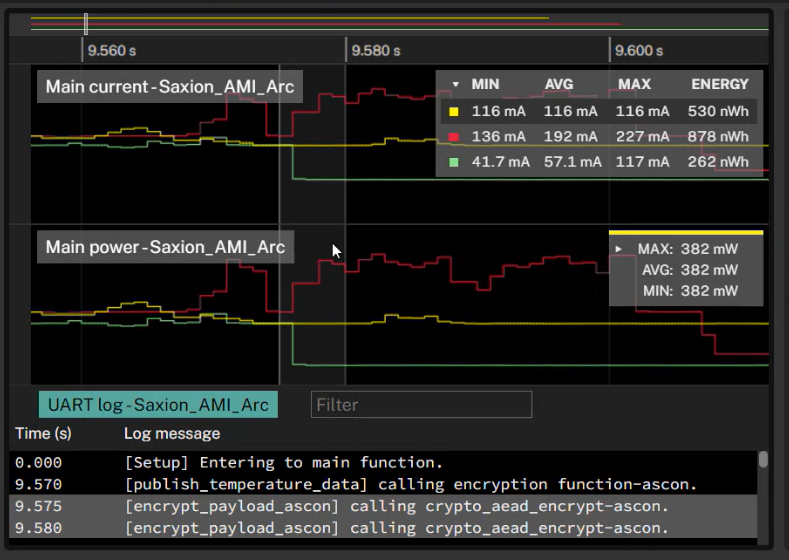
\includegraphics[width=0.9\linewidth]{images/fp/power-otti.png}
    \caption{Power Analysis Read of LOLIN32 Lite ESP32 Using Otii-arch Device.}
    \label{fig:otii-mon}
\end{figure}

Figure \ref{fig:otii-mon} shows the power consumption results of three implementations (no-encryption-green, ASCON-yello, and AES-GCM-red). At around 9.56 seconds, the power consumption of the three implementations is approximately equal. However, as time progresses, the power consumption of AES-GCM increases significantly, while the power consumption of ASCON remains relatively constant at around 116 mA. This suggests that the AES-GCM algorithm requires more CPU cycles than ASCON, which results in a higher power spike.

